\section{Distributed crawling(splitting by key range vs. hash of key)}
This section presents strategies to distribute crawling activity across many nodes. Each participating
node is given the responsibility of downloading a slice of seed set. The main reason to distribute
crawling is to make it scalable.  
\\
\\
Mercator's\cite{mercator}(1999) host splitter component distributes load by hostname. Limitations of this way of distribution and alternatives are discussed below. Ubicrawler\cite{ubicrawler}(2004) achieved linear scalability, fault tolerance through consistent hashing\cite{consisthash}. Both designs mention some form of
load balancing however papers fall short of explanation on technicalities surrounding it.
\\
\\
When the goal is to distribute load evenly across nodes, say, 5 nodes should handle 5 times the throughput
of a single node. One way to split the load is to assign a range of request boundaries from minimum to
maximum to each node. Examples for range of keys can be based on hostname, alphabets A-Z, etc. This works
as long as there exist calculated risk of every node getting a fair share of the load but in many cases,
load is unbalanced which causes one crawler node to compute more data than others causing skewed
workloads\cite{consisthash}. In extreme cases, only a specific boundary(e.g A-D) assigned to a node is taking all the node while other node(e.g X-Z) sits idle, such high disproportionate load is said to be a hot spot\cite{consisthash} in distributed systems terminology.
\\
\\
An alternative to distributing load by key range is to use hash function such that output of hash of a key
is an integer which maps to a position somewhere on the line across the range of numbers, shown in figure \ref{fig:requestboundary}. A hash function with low collision probability can turn a skewed load into uniformly distributed load. Figure \ref{fig:requestboundary} shows a 16-bit hash function that can return a
random number between $0$ to $2^N-1$.
\begin{figure}[h!]
  \centering
  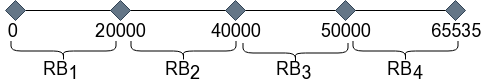
\includegraphics[width=10cm,height=4cm,keepaspectratio]{../media/crawler/requestboundaries.png}
  \caption{partitioning by hash of key}
  \label{fig:requestboundary}
\end{figure}

\pagebreak

\noindent
Such a hash function is used to assign a node(physical machine) a range of hash values. Certain attributes of a machine can be used as a input key to a hash function mapping to a integer on the line figure \ref{fig:modnsplit}. From left to right, when hash of a absolute URL(e.g at 23000) used as a key falls within a nodes range, task request is fulfilled by that node(at 40000). This way of distributing the load evenly across
machine is called consistent hashing\cite{consisthash}. Hashing reduces skewed workloads and hot spots
but they cannot be 100 percent eliminated.

\begin{figure}[h!]
  \centering
  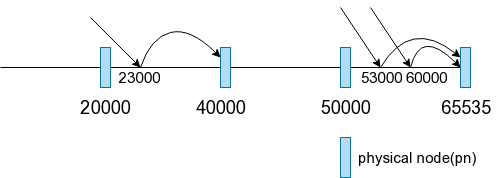
\includegraphics[width=10cm,height=4cm,keepaspectratio]{../media/crawler/modnsplit.png}
  \caption{Rebalancing physical nodes by mod N}
  \label{fig:modnsplit}
\end{figure}

\begin{figure}[h!]
  \centering
  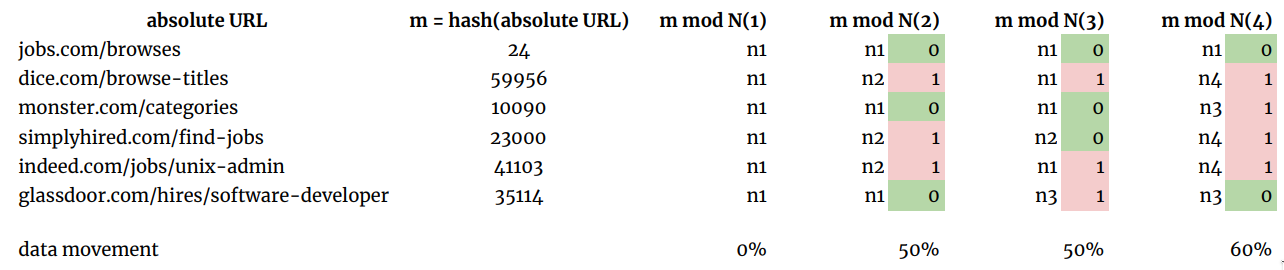
\includegraphics[width=16cm,height=8cm,keepaspectratio]{../media/crawler/modn_info.png}
  \caption{data movement when using modulo N}
  \label{fig:movemodn}
\end{figure}

\begin{figure}[h!]
  \centering
  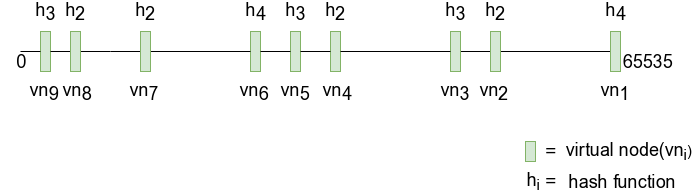
\includegraphics[width=12cm,height=5cm,keepaspectratio]{../media/crawler/vnodesplit1.png}
  \caption{virtual nodes to reduce shifts in data movements between nodes}
  \label{fig:vnodesplit1}
\end{figure}

\begin{figure}[h!]
  \centering
  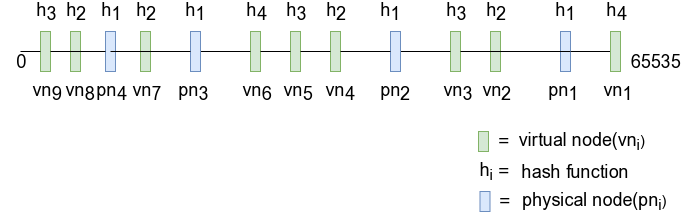
\includegraphics[width=12cm,height=5cm,keepaspectratio]{../media/crawler/vnodesplit2.png}
  \caption{Rebalancing physical nodes with virtual nodes}
  \label{fig:vnodesplit2}
\end{figure}

\begin{figure}[h!]
  \centering
  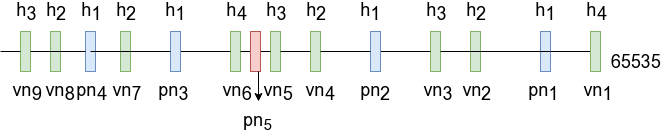
\includegraphics[width=12cm,height=5cm,keepaspectratio]{../media/crawler/addingnode.png}
  \caption{adding new node to existing cluster of nodes}
  \label{fig:addingnode}
\end{figure}

\begin{figure}[h!]
  \centering
  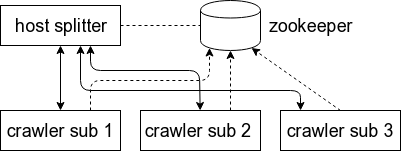
\includegraphics[width=8cm,height=5cm,keepaspectratio]{../media/crawler/zookeeper.png}
  \caption{zookeeper used to maintain up-to-date information on which vnodes are assigned to pnodes}
  \label{fig:zookeeper}
\end{figure}

\begin{figure}[h!]
  \centering
  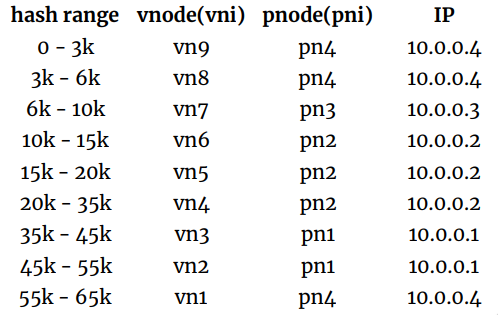
\includegraphics[width=10cm,height=8cm,keepaspectratio]{../media/crawler/zookeeper_info.png}
  \caption{zookeeper table}
  \label{fig:zookeeper_info}
\end{figure}

\pagebreak
